\documentclass[12pt,a4paper]{article}
\author{}
\date{}
\title{Mueller Plathe's Stimulation}
\usepackage{amsmath}
\usepackage{graphicx}
\begin{document}
\maketitle
\section{}
\subsection*{} 
\begin{figure}[h]
  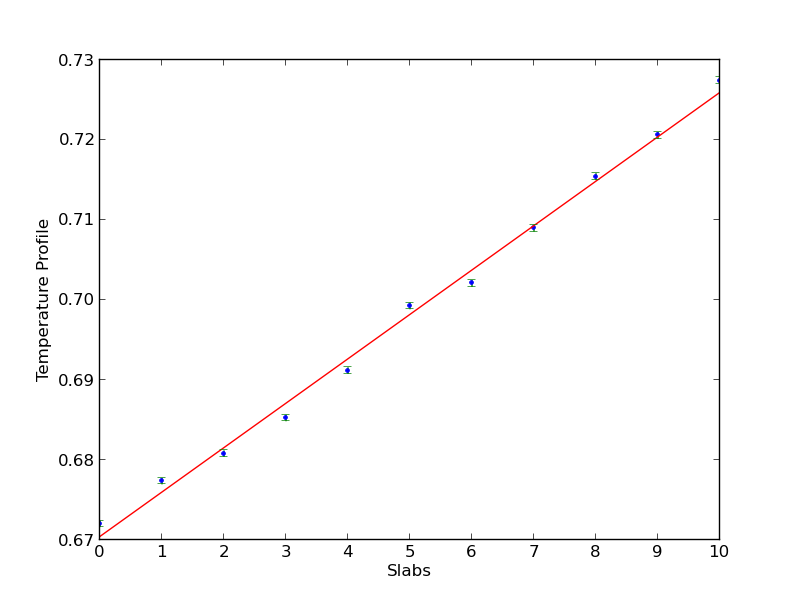
\includegraphics[width=\linewidth]{TemperatureProfile.png}
\end{figure}
\begin{align*}
 \kappa &= 7.045 \\
 \sigma_\kappa&=0.168
\end{align*}
\subsection*{}
\begin{figure}[!htb]
  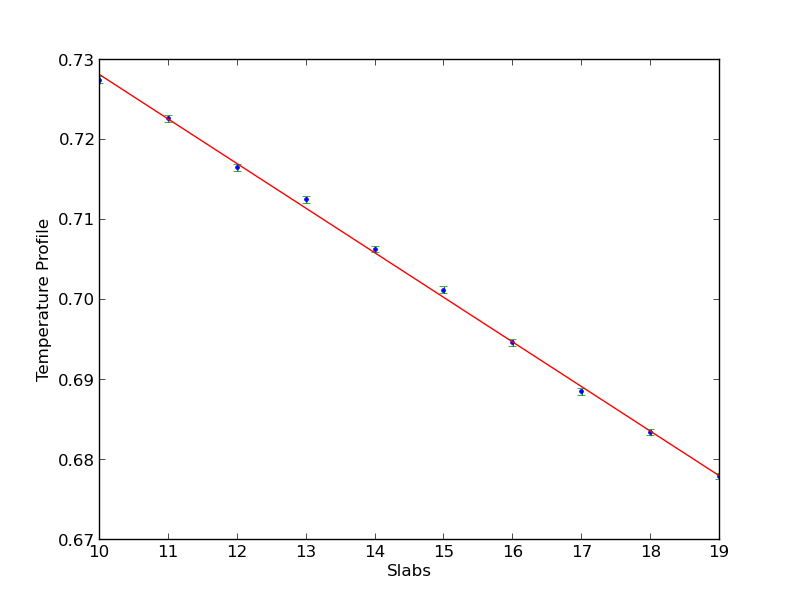
\includegraphics[width=\linewidth]{TemperatureProfile-.png}
\end{figure}
\begin{align*}
\kappa &=7.016  \\
\sigma_\kappa &=0.0901
\end{align*}
\newpage
\section{}
\begin{figure}[!htb]
\minipage{0.6\textwidth}
  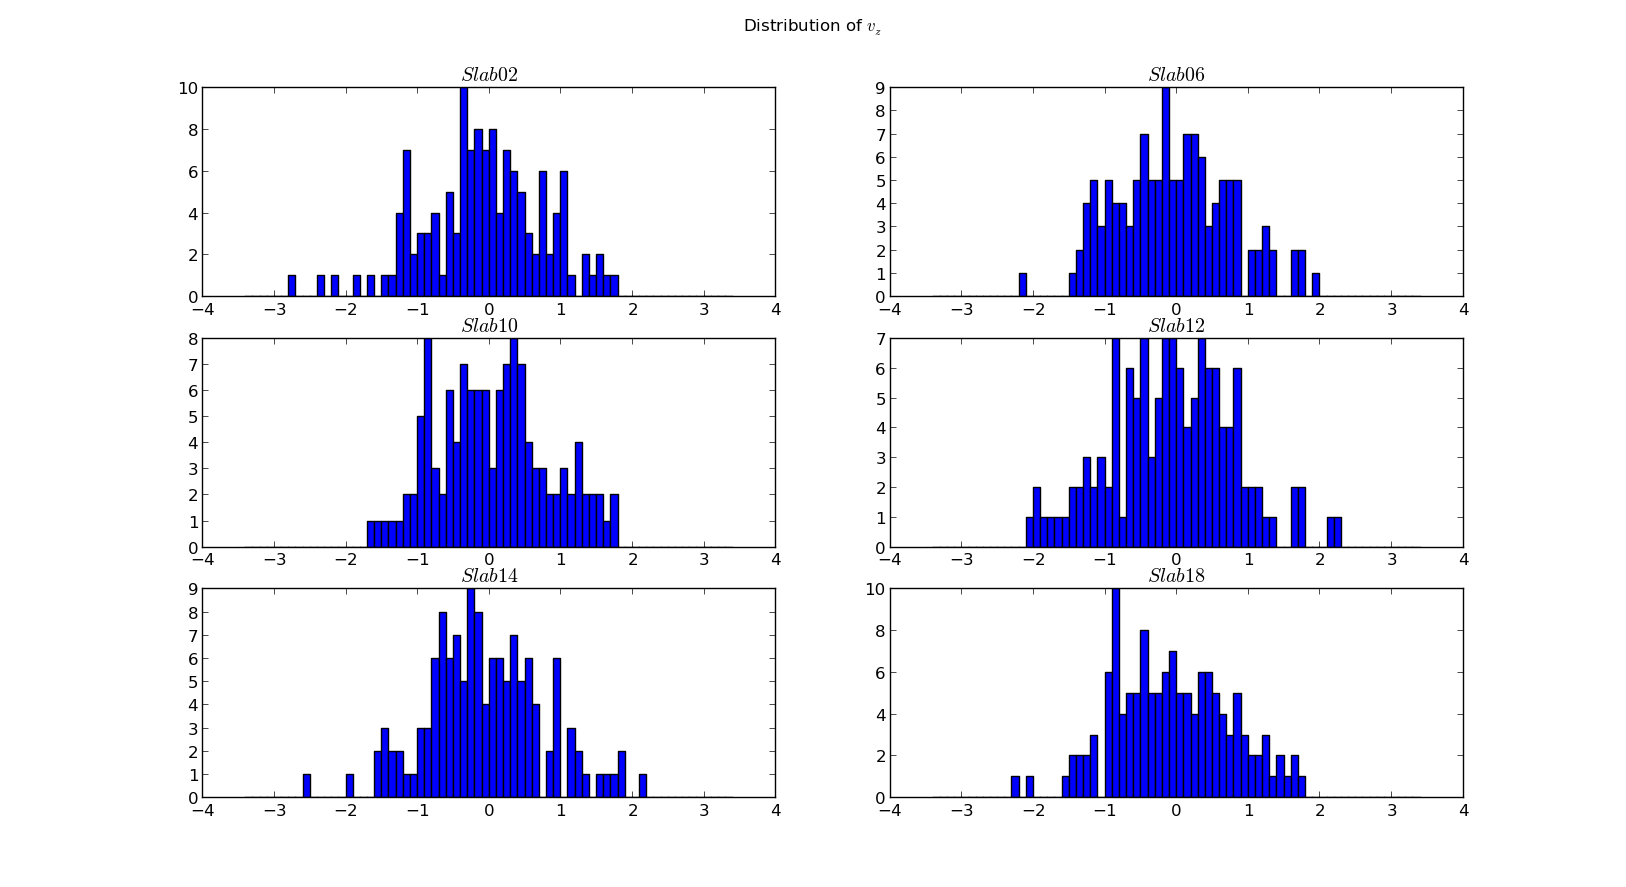
\includegraphics[width=\linewidth]{fVx.png}
  %\caption{$e$ neutrino oscillations, long range.}\label{fig:awesome_image1}
\endminipage\hfill
\minipage{0.6\textwidth}
  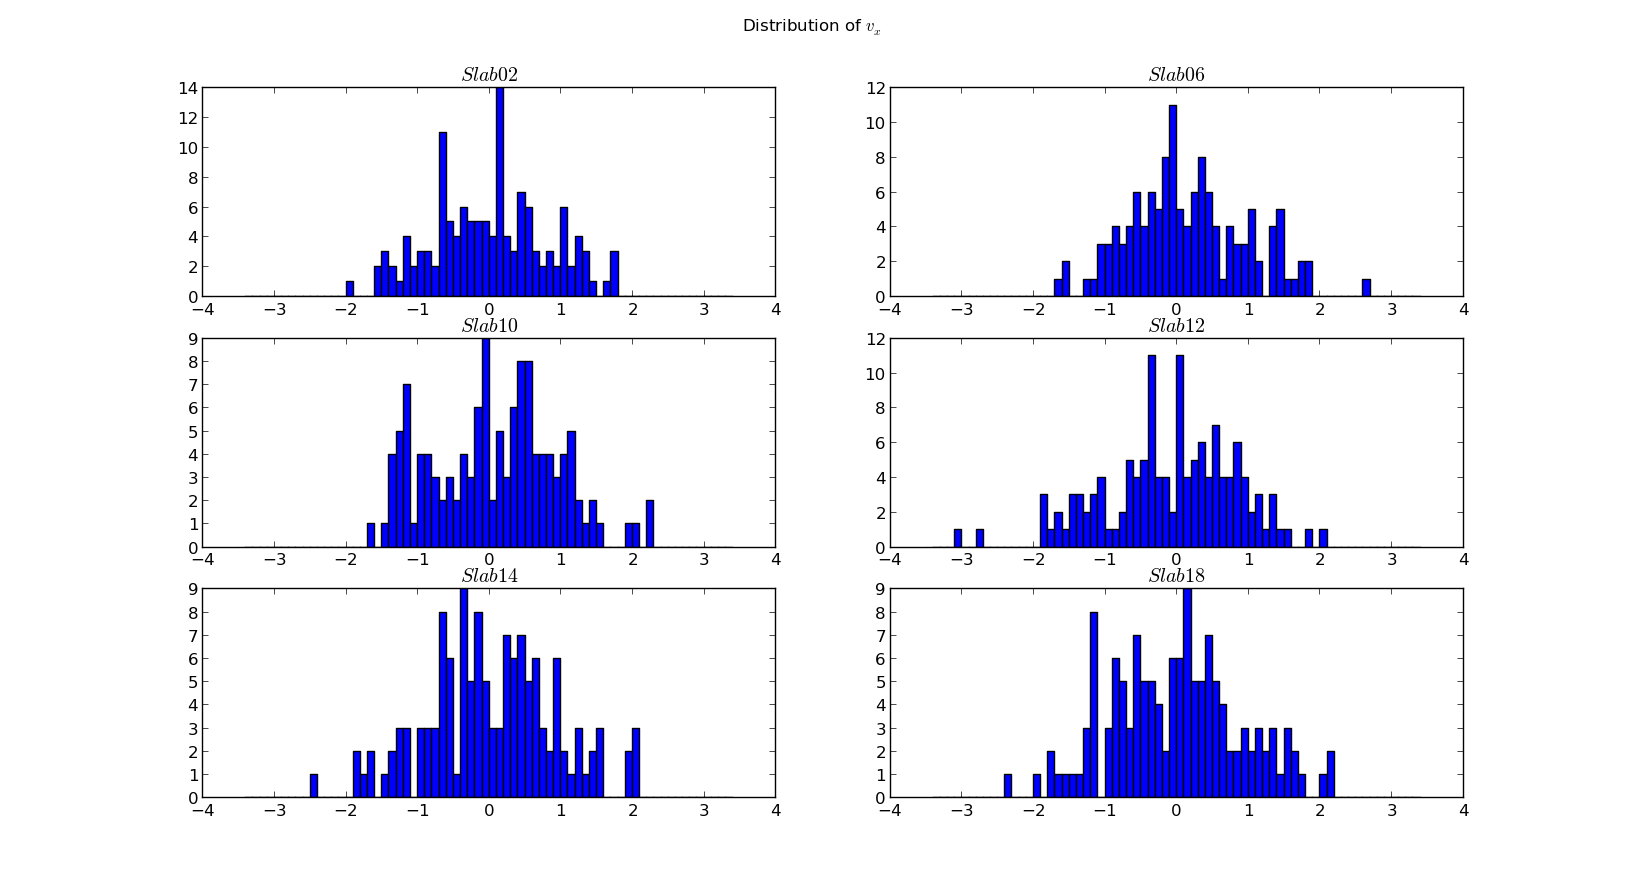
\includegraphics[width=\linewidth]{fVz.png}
 % \caption{$\mu$ neutrino oscillations, long range.}\label{fig:awesome_image2}
\endminipage\hfill
\end{figure}

\begin{figure}[h]
\centering
  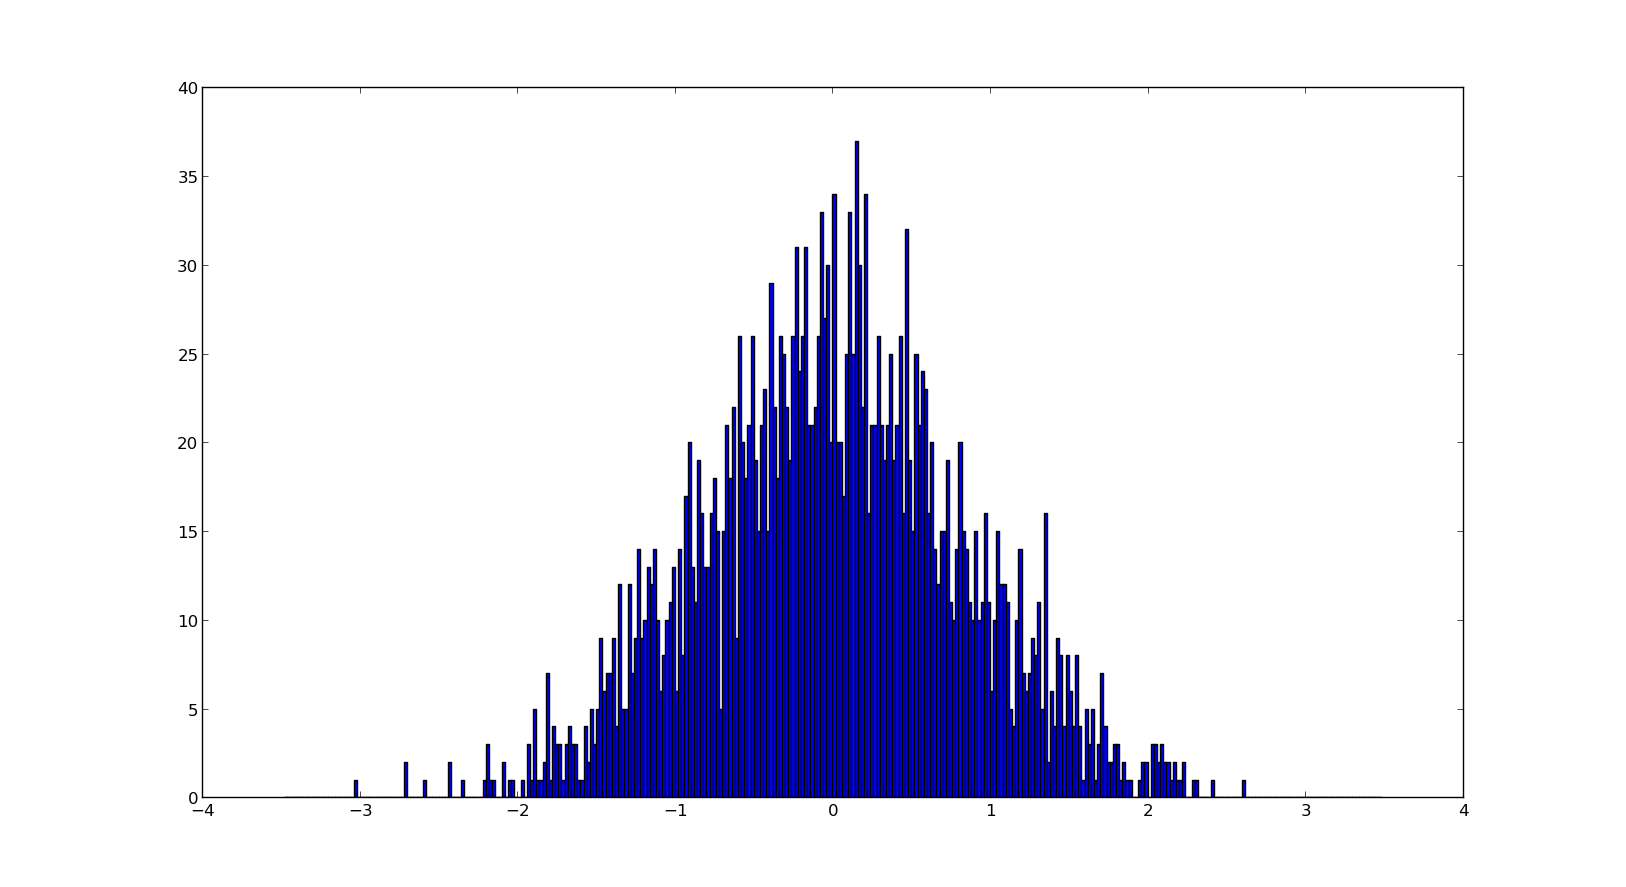
\includegraphics[width=0.6\linewidth]{fsystem.png}
\end{figure}
\section{}
\begin{figure}[!htb]
\minipage{0.6\textwidth}
  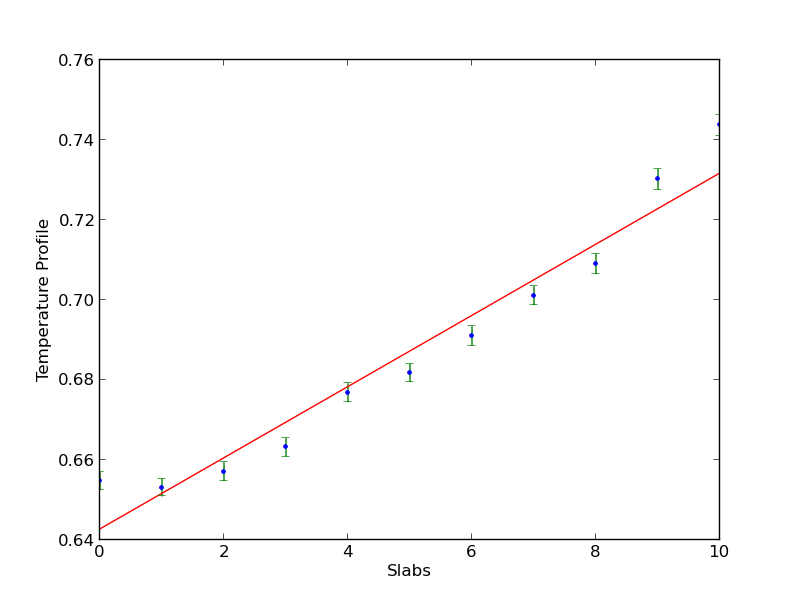
\includegraphics[width=\linewidth]{1.png}
  %\caption{$e$ neutrino oscillations, long range.}\label{fig:awesome_image1}
\endminipage\hfill
\minipage{0.6\textwidth}
  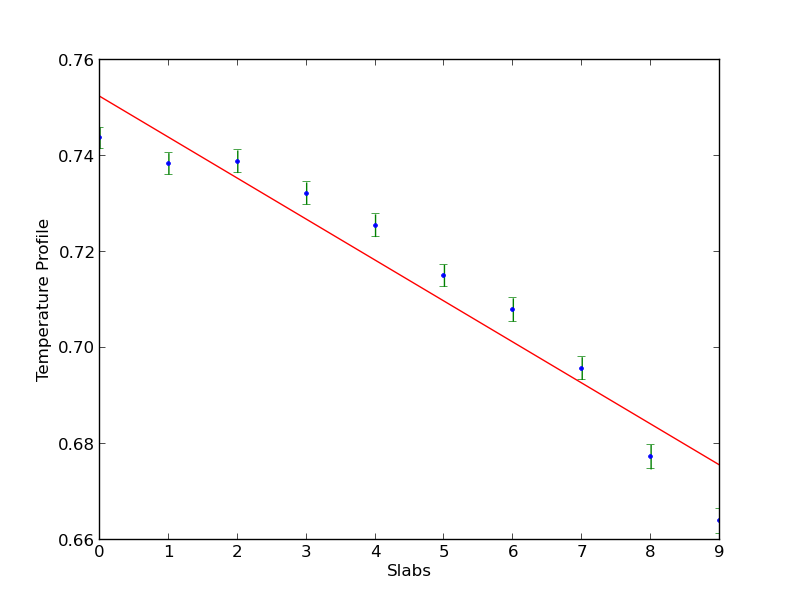
\includegraphics[width=\linewidth]{2.png}
 % \caption{$\mu$ neutrino oscillations, long range.}\label{fig:awesome_image2}
\endminipage\hfill
\end{figure}
\end{document}